\chapter{Anexo}


\clearpage
\pagestyle{empty}
\newgeometry{left=3mm,right=3mm,top=3mm,bottom=3mm,}

\section{simulaciones}

  \begin{figure}[H]
    \centering
    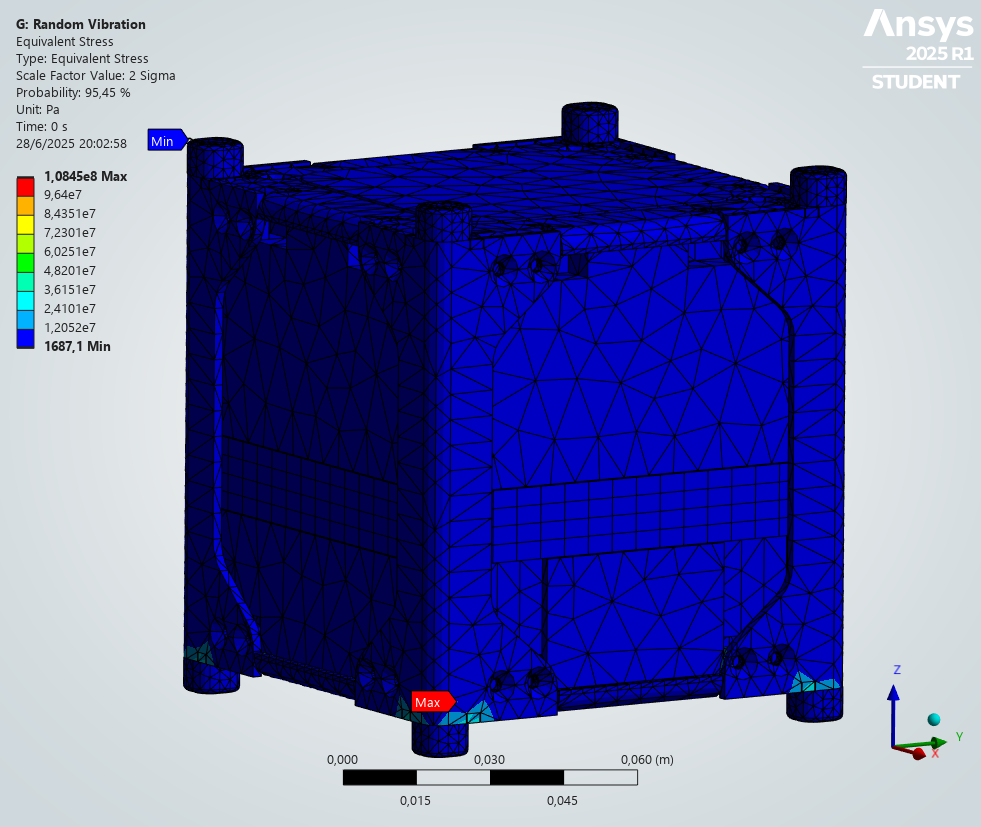
\includegraphics[width=15cm]{image/fem/ansys_cubesat-vibration_stress.png}
    \caption{Analisis de estres}
    \label{fig:fem_stress}
  \end{figure}

  \begin{figure}[H]
    \centering
    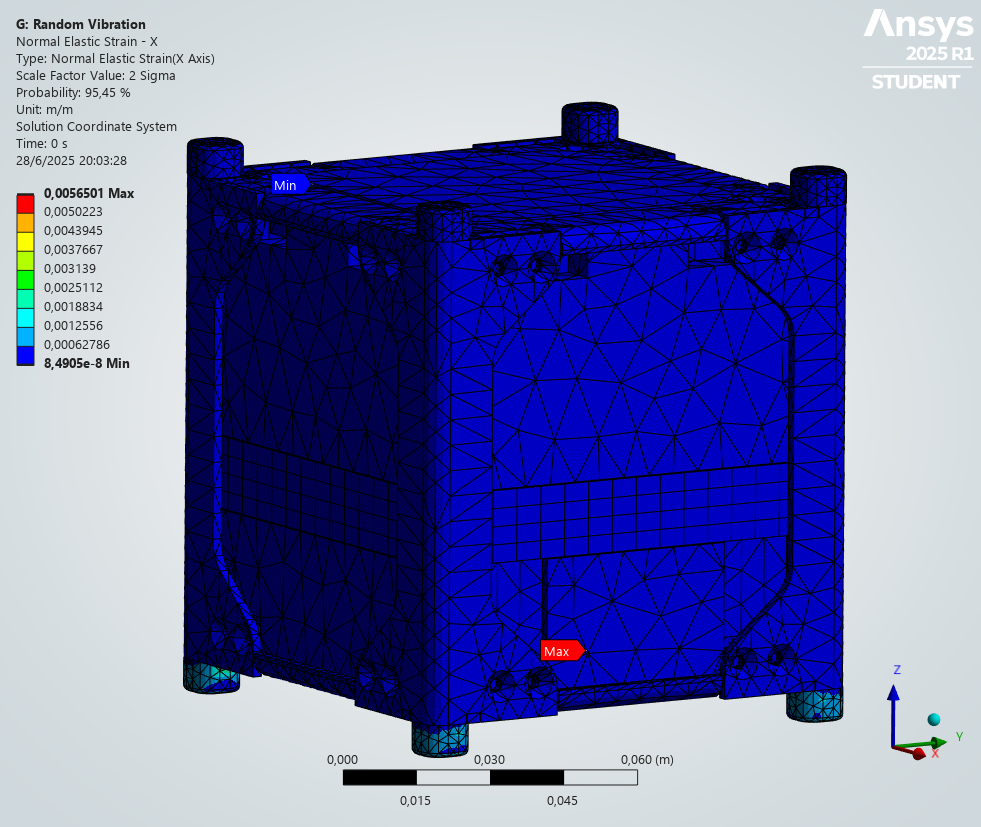
\includegraphics[width=14cm]{image/fem/ansys_cubesat-vibration_strain-x.png}
    \caption{Analisis de tensión en el eje x}
    \label{fig:fem_strain-x}
  \end{figure}

  \begin{figure}[H]
    \centering
    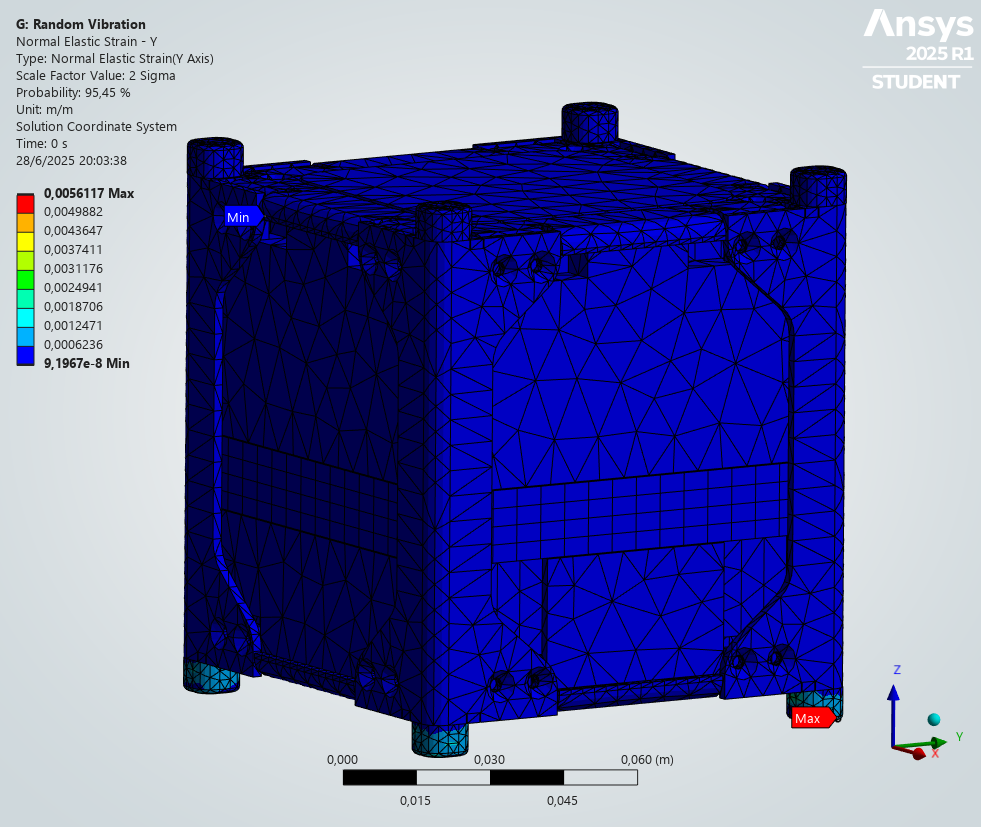
\includegraphics[width=14cm]{image/fem/ansys_cubesat-vibration_strain-y.png}
    \caption{Analisis de tensión en el eje Y}
    \label{fig:fem_strain-y}
  \end{figure}

  \begin{figure}[H]
    \centering
    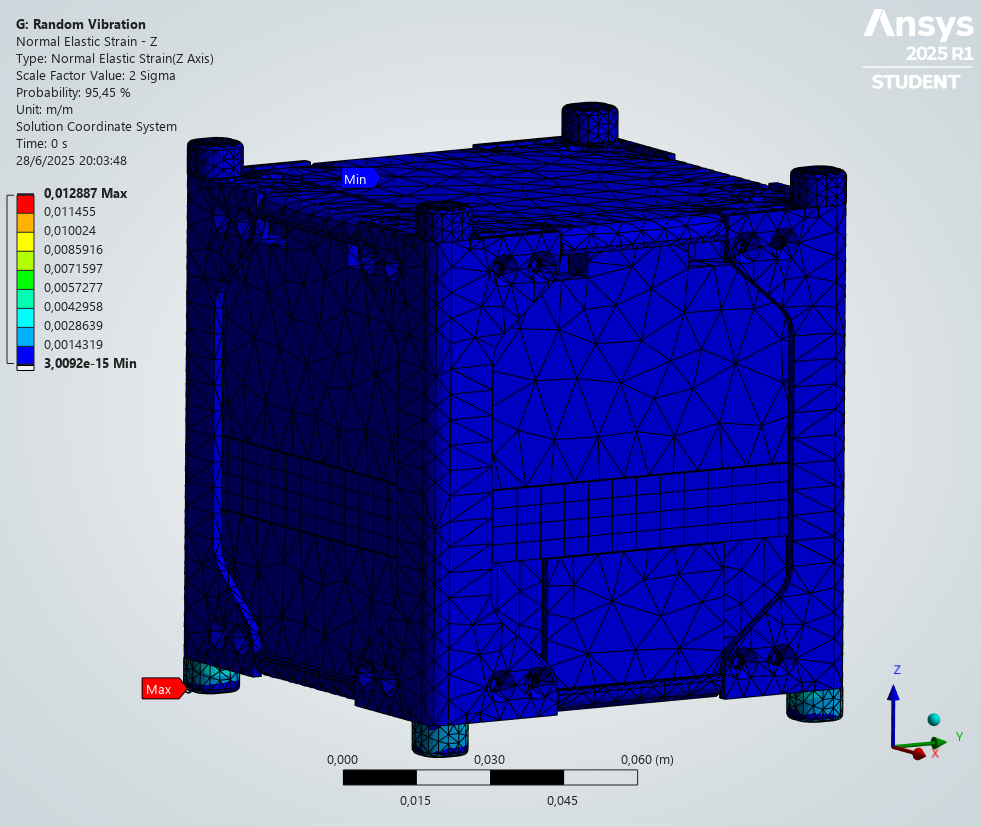
\includegraphics[width=14cm]{image/fem/ansys_cubesat-vibration_strain-z.png}
    \caption{Analisis de tensión en el eje Z}
    \label{fig:fem_strain-z}
  \end{figure}

  \begin{figure}[H]
    \centering
    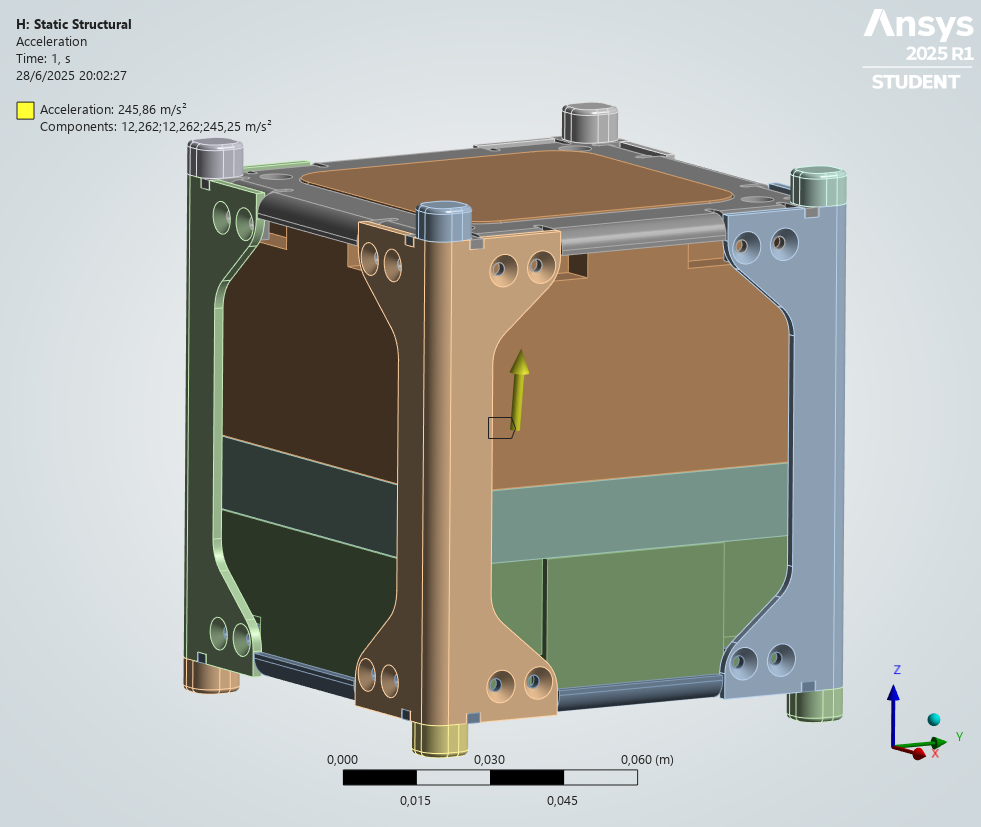
\includegraphics[width=14cm]{image/fem/ansys_cubesat-static_acceleration.png}
    \caption{Vector de aceleración para la simulación estática.}
    \label{fig:fem_static_acc}
  \end{figure}

  \begin{figure}[H]
    \centering
    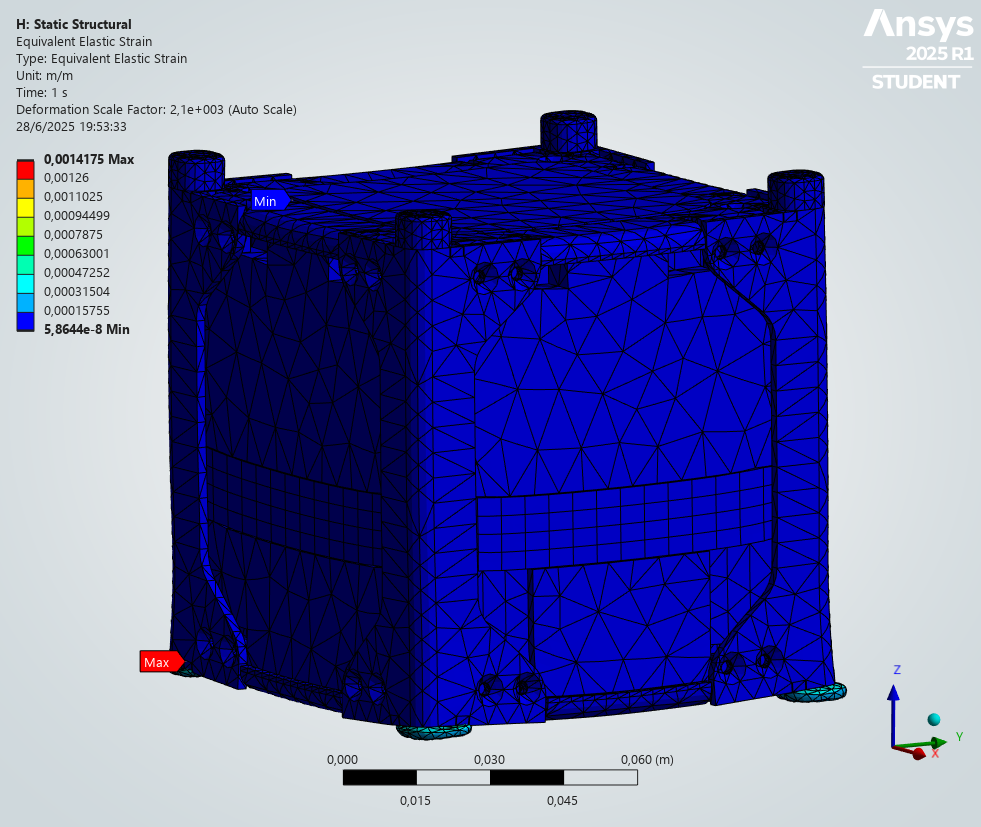
\includegraphics[width=14cm]{image/fem/ansys_cubesat-static_strain.png}
    \caption{Analisis de fatiga}
    \label{fig:fem_static_strain}
  \end{figure}

  \begin{figure}[H]
    \centering
    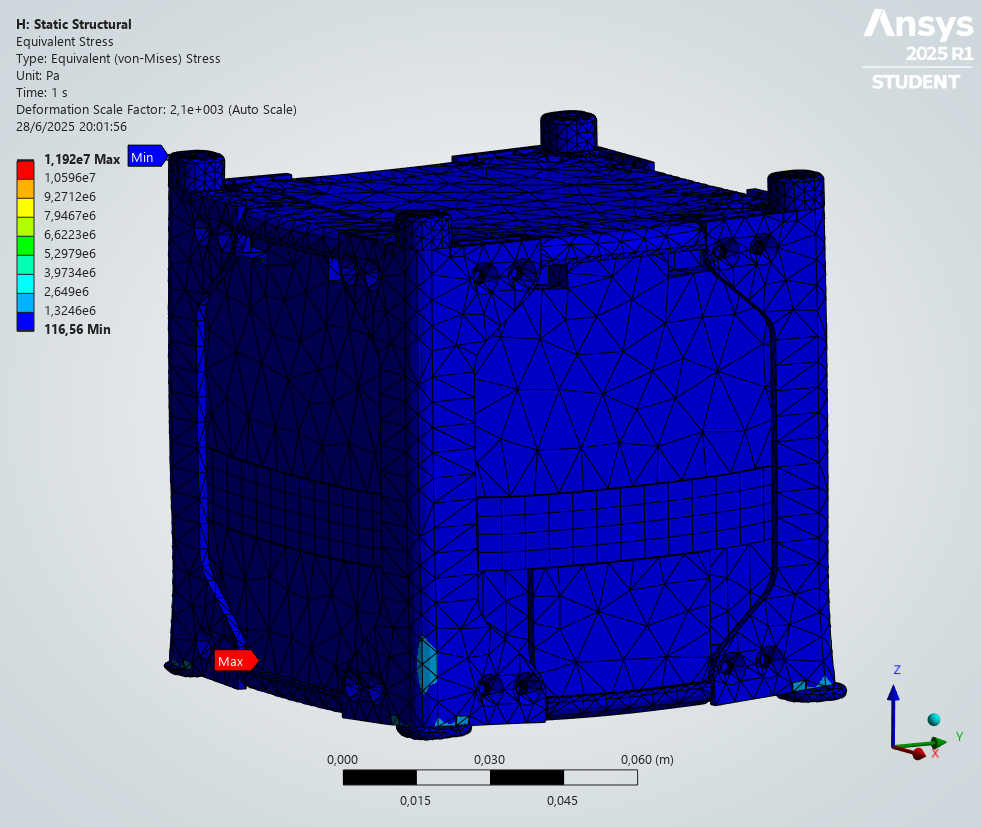
\includegraphics[width=14cm]{image/fem/ansys_cubesat-static_stress.png}
    \caption{Analisis de estrés}
    \label{fig:fem_static_stress}
  \end{figure}

  \begin{figure}[H]
    \centering
    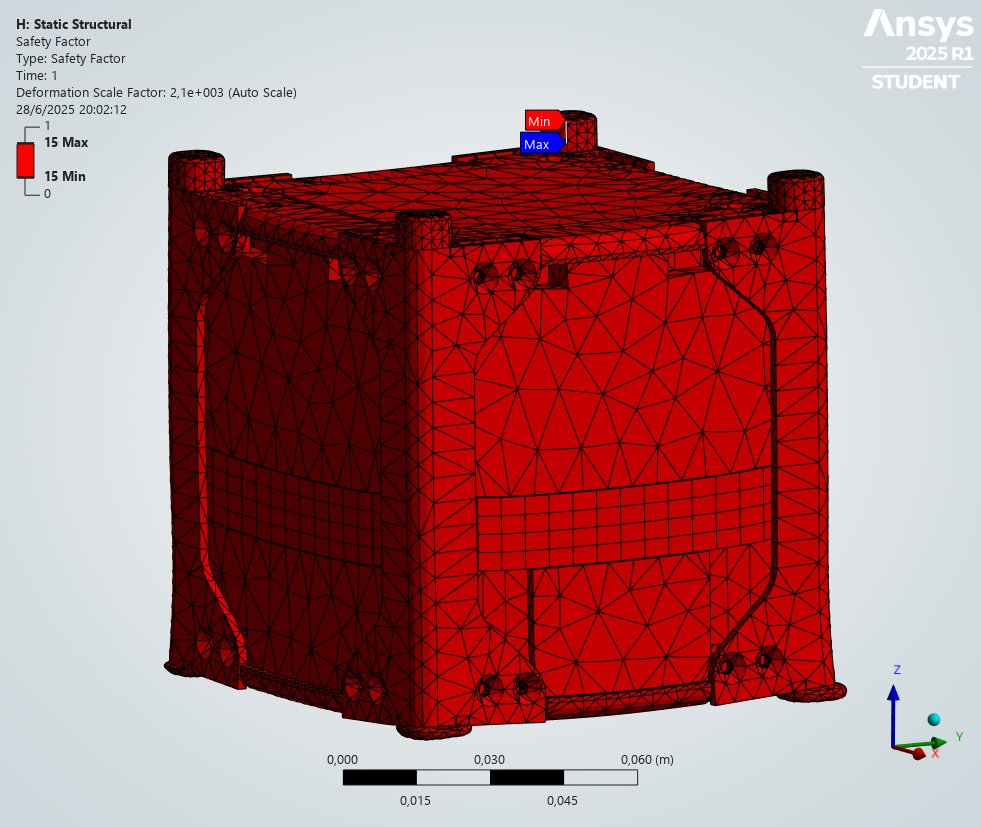
\includegraphics[width=14cm]{image/fem/ansys_cubesat-static_safety.png}
    \caption{Analisis de factor de seguridad}
    \label{fig:fem_static_safety}
  \end{figure}

  \begin{figure}[H]
    \centering
    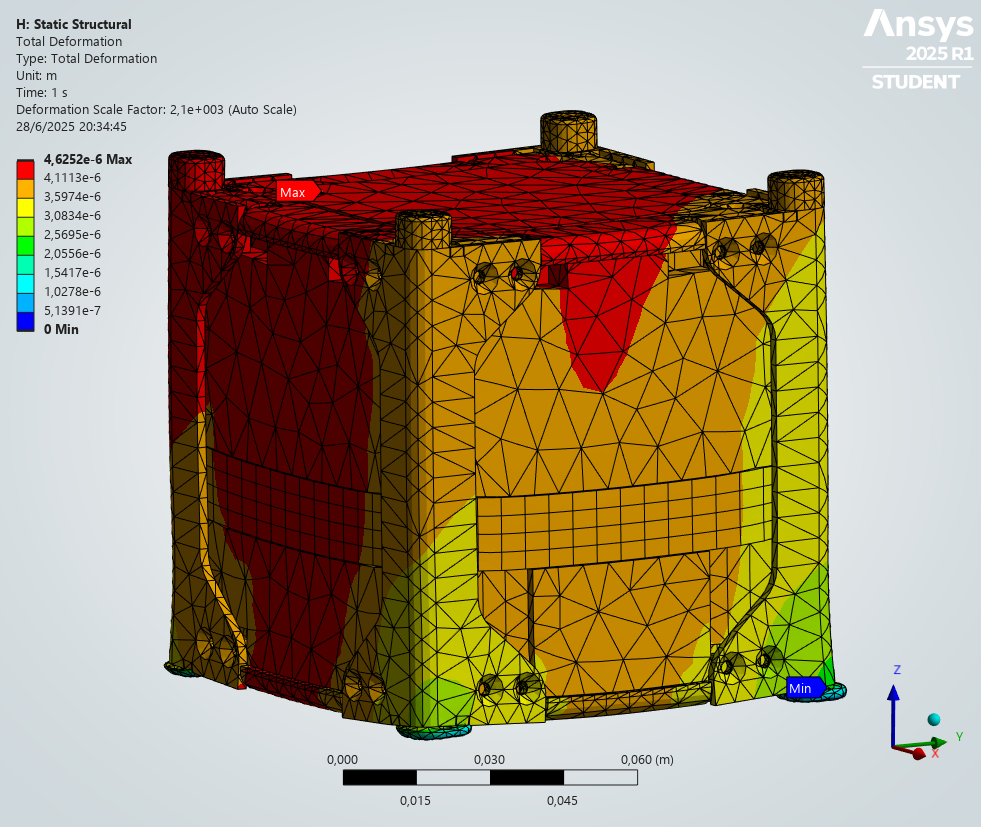
\includegraphics[width=14cm]{image/fem/ansys_cubesat-static_deformation.png}
    \caption{Analisis de deformación total}
    \label{fig:fem_static_deformation}
  \end{figure}

\begin{landscape}
\section{Cronograma Electrónica}

 \begin{figure}[H]
  \centering
  \resizebox{25cm}{!}{%
  \begin{ganttchart}[
    hgrid,
    vgrid,
    time slot format=isodate,
    x unit=0.65cm,
    y unit chart=1cm,
    bar/.append style={fill=blue!40},
    milestone/.append style={fill=orange},
    milestone label font=\bfseries\small,
    bar label font=\small\slshape
    ]{2025-07-04}{2025-08-31}

  % July
  \gantttitlecalendar{month=name,week,day} \\

  % Tasks
  \ganttgroup{Validación de Subsistemas}{2025-07-04}{2025-07-09} \\
  \ganttbar[name=rev-pcb]{Revisión de PCB}{2025-07-04}{2025-07-09} \\
  \ganttbar[name=rev-sensores]{Revisión de Sensores}{2025-07-04}{2025-07-09} \\

  \ganttgroup{CAD Computadora de Vuelo}{2025-07-10}{2025-07-17} \\
  \ganttbar[name=diseño-esq1]{Diseño esquemático}{2025-07-10}{2025-07-12} \\
  \ganttlinkedbar{Diseño PCB}{2025-07-13}{2025-07-16} \\
  \ganttlinkedmilestone[name=team-meating1]{Team Meeting}{2025-07-17} \\
  \ganttlink{rev-pcb}{diseño-esq1}
  \ganttlink[link mid=.25]{rev-sensores}{diseño-esq1}
  
  \ganttgroup{CAD PMS}{2025-07-18}{2025-07-24} \\
  \ganttbar[name=diseño-esq2]{Diseño esquemático}{2025-07-18}{2025-07-20} \\
  \ganttlinkedbar{Diseño PCB}{2025-07-20}{2025-07-23} \\
  \ganttlinkedmilestone[name=team-meating2]{Team Meeting}{2025-07-24} \\ 
  \ganttlink[link mid=.25]{team-meating1}{diseño-esq2}

  \ganttgroup{CAD TRU}{2025-07-25}{2025-07-31} \\
  \ganttbar[name=diseño-esq3]{Diseño esquemático}{2025-07-25}{2025-07-27} \\
  \ganttlinkedbar{Diseño PCB}{2025-07-27}{2025-07-30} \\
  \ganttlinkedmilestone{Team Meeting}{2025-07-31} \\
  \ganttlink[link mid=.25]{team-meating2}{diseño-esq3}

  \ganttlinkedbar{Prototipo Mínimo Funcional}{2025-08-01}{2025-08-07} \\
  \ganttlinkedmilestone[name=entrega-cdr]{Entrega CDR}{2025-08-08} \\

  \ganttgroup{Construcción 1ra versión}{2025-08-09}{2025-08-18} \\
  \ganttbar[name=planchado]{Planchado de PCBs}{2025-08-09}{2025-08-11} \\
  \ganttlinkedbar{Soldado de componentes}{2025-08-12}{2025-08-12} \\
  \ganttlinkedbar[name=test-points]{Verificación de test points}{2025-08-13}{2025-08-14} \\
  \ganttlinkedbar{Interconexión de sistemas}{2025-08-15}{2025-08-18} \\
  \ganttbar[name=iden-errores]{Identificación de errores}{2025-08-15}{2025-08-18} \\
  \ganttlink[link mid=.25]{test-points}{iden-errores}  
  \ganttlink[link mid=.25]{entrega-cdr}{planchado}

  \ganttgroup{Construcción Producto Final}{2025-08-19}{2025-08-31} \\
  \ganttbar[name=planchado2]{Planchado de PCB}{2025-08-19}{2025-08-22} \\
  \ganttlink[link mid=.25]{iden-errores}{planchado2} 
  \ganttlinkedbar[name=soldado]{Soldado}{2025-08-23}{2025-08-24} \\
  \ganttlinkedbar[name=func-conj]{Funcionamiento en conjunto}{2025-08-24}{2025-08-31} \\
  \ganttbar[name=iden-fallas]{Identificación de posibles fallas}{2025-08-24}{2025-08-31} \\

  \ganttlink[link mid=.25]{soldado}{iden-fallas}
  \end{ganttchart}
  }
  \end{figure}

  \section{Cronograma software}
    \begin{figure}[H]
      \centering
      \resizebox{25cm}{!}{%
        \begin{ganttchart}[
        hgrid,
        vgrid,
        time slot format=isodate,
        x unit=0.65cm,
        y unit chart=0.65cm,
        bar/.append style={fill=blue!40},
        milestone/.append style={fill=orange},
        milestone label font=\bfseries\small,
        bar label font=\small\slshape
    ]{2025-07-06}{2025-08-17}

      \gantttitlecalendar{month=name, week, day} \\

      %\ganttlink{req}{tools}
      %\ganttlink{tools}{design}
      %\ganttlink{design}{developpdr}
      %\ganttlink{developpdr}{delivpdr}

      \ganttgroup{Desarrollo de CDR}{2025-07-08}{2025-08-08} \\
      \ganttbar{Evaluación y revisión de correcciones}{2025-07-08}{2025-08-07} \\
      \ganttbar{Desarrollo de CDR}{2025-07-08}{2025-08-07} \\
      \ganttlinkedmilestone[name=delivcdr]{Entrega de CDR}{2025-08-08} \\

      \ganttgroup{Selección de equipo}{2025-08-09}{2025-08-14} \\
      \ganttbar{Evaluación}{2025-08-09}{2025-08-13} \\
      \ganttbar{Selección}{2025-08-14}{2025-08-14} \\

      \ganttgroup{Diseño de software}{2025-07-06}{2025-07-09} \\
      \ganttbar{Especificación de funcionalidades}{2025-07-06}{2025-07-09} \\
      \ganttbar{Diseño del sistema}{2025-07-06}{2025-07-09} \\

      \ganttgroup{Configuración de entorno}{2025-07-10}{2025-07-19} \\
      \ganttbar{Configuración del sistema operativo}{2025-07-10}{2025-07-14} \\
      \ganttbar{Instalación de herramientas}{2025-07-10}{2025-07-14} \\
      \ganttbar{Configuración de acceso}{2025-07-13}{2025-07-19} \\

      \ganttgroup{Integración de sensores}{2025-07-20}{2025-07-24} \\
      \ganttbar{Integración con lectura de sensores}{2025-07-20}{2025-07-22} \\
      \ganttbar{Compresión de datos}{2025-07-23}{2025-07-24} \\

      \ganttgroup{Sprint 1}{2025-07-25}{2025-08-17}\\

      \ganttgroup{Desarrollo backend}{2025-07-25}{2025-08-13} \\
      \ganttbar{Desarrollo de funcionalidades principales}{2025-07-25}{2025-07-31} \\
      \ganttbar{Análisis de datos}{2025-07-28}{2025-08-03} \\
      \ganttbar{Generación de reportes}{2025-08-04}{2025-08-08} \\
      \ganttbar{Manejo de errores}{2025-08-09}{2025-08-13} \\
      \ganttbar{Administración de logs}{2025-08-09}{2025-08-13} \\

      \ganttgroup{Almacenamiento}{2025-07-27}{2025-08-02} \\
      \ganttbar{Almacenamiento de datos}{2025-07-27}{2025-08-02} \\
      \ganttbar{Implementación RAID 1}{2025-07-27}{2025-08-02} \\

      \ganttgroup{Desarrollo frontend}{2025-08-04}{2025-08-10} \\
      \ganttbar{Interfaz visual}{2025-08-04}{2025-08-10} \\

      \ganttgroup{Testing}{2025-08-14}{2025-08-17} \\
      \ganttbar{Pruebas unitarias funcionales}{2025-08-14}{2025-08-15} \\
      \ganttbar{Pruebas unitarias no funcionales}{2025-08-14}{2025-08-15} \\
      \ganttbar{Pruebas de estrés}{2025-08-14}{2025-08-15} \\
      \ganttbar{Validación de hardware}{2025-08-16}{2025-08-17} \\
      \ganttbar{Corrección de posibles fallos}{2025-08-14}{2025-08-17} \\

    \end{ganttchart}
    }
    \end{figure}

  \newpage
  \section{Cronograma software}
    \begin{figure}[H]
      \centering
      \resizebox{25cm}{!}{%
        \begin{ganttchart}[
        hgrid,
        vgrid,
        time slot format=isodate,
        x unit=0.65cm,
        y unit chart=0.65cm,
        bar/.append style={fill=blue!40},
        milestone/.append style={fill=orange},
        milestone label font=\bfseries\small,
        bar label font=\small\slshape
    ]{2025-08-18}{2025-10-10}

      \gantttitlecalendar{month=name, week, day} \\

      %\ganttlink{req}{tools}
      %\ganttlink{tools}{design}
      %\ganttlink{design}{developpdr}
      %\ganttlink{developpdr}{delivpdr}

      \ganttgroup{Sprint 2}{2025-08-18}{2025-09-10}\\

      \ganttgroup{Desarrollo backend}{2025-08-18}{2025-09-06} \\
      \ganttbar{Desarrollo de funcionalidades principales}{2025-08-18}{2025-08-24} \\
      \ganttbar{Análisis de datos}{2025-08-21}{2025-08-27} \\
      \ganttbar{Generación de reportes}{2025-08-28}{2025-09-01} \\
      \ganttbar{Manejo de errores}{2025-09-02}{2025-09-06} \\
      \ganttbar{Administración de logs}{2025-09-02}{2025-09-06}\\

      \ganttgroup{Almacenamiento}{2025-08-20}{2025-08-26} \\
      \ganttbar{Almacenamiento de datos}{2025-08-20}{2025-08-26} \\
      \ganttbar{Implementación RAID 1}{2025-08-20}{2025-08-26}\\

      \ganttgroup{Desarrollo frontend}{2025-08-28}{2025-09-03} \\
      \ganttbar{Interfaz visual}{2025-08-28}{2025-09-03} \\

      \ganttgroup{Testing}{2025-09-07}{2025-09-10}  \\
      \ganttbar{Pruebas unitarias funcionales}{2025-09-07}{2025-09-08} \\
      \ganttbar{Pruebas unitarias no funcionales}{2025-09-07}{2025-09-08}  \\
      \ganttbar{Pruebas de estrés}{2025-09-07}{2025-09-08}  \\
      \ganttbar{Validación de hardware}{2025-09-09}{2025-09-10}  \\
      \ganttbar{Corrección de posibles fallos}{2025-09-07}{2025-09-10}  \\

      \ganttgroup{Sprint 3}{2025-09-11}{2025-10-04}\\

       \ganttgroup{Desarrollo backend}{2025-09-11}{2025-09-20} \\\ganttbar{Desarrollo de funcionalidades principales}{2025-09-11}{2025-09-17} \\
      \ganttbar{Análisis de datos}{2025-09-14}{2025-09-20} \\
      \ganttbar{Generación de reportes}{2025-09-21}{2025-09-25} \\
      \ganttbar{Manejo de errores}{2025-09-26}{2025-09-30} \\
      \ganttbar{Administración de logs}{2025-09-26}{2025-09-30} \\

      \ganttgroup{Almacenamiento}{2025-09-13}{2025-09-19} \\
      \ganttbar{Almacenamiento de datos}{2025-09-13}{2025-09-19} \\
      \ganttbar{Implementación RAID 1}{2025-09-13}{2025-09-19} \\

      \ganttgroup{Desarrollo frontend}{2025-09-21}{2025-09-27} \\
      \ganttbar{Interfaz visual}{2025-09-21}{2025-09-27} \\

      \ganttgroup{Testing}{2025-10-01}{2025-10-04} \\
      \ganttbar{Pruebas unitarias funcionales}{2025-10-01}{2025-10-02} \\
      \ganttbar{Pruebas unitarias no funcionales}{2025-10-01}{2025-10-02} \\
      \ganttbar{Pruebas de estrés}{2025-10-01}{2025-10-02} \\
      \ganttbar{Validación de hardware}{2025-10-03}{2025-10-04} \\
      \ganttbar{Corrección de posibles fallos}{2025-10-01}{2025-10-04} \\

      \ganttlinkedmilestone[name=delivcdr]{Entrega final}{2025-10-10}

      \end{ganttchart}
      }
    \end{figure}

\end{landscape}
\restoregeometry
\setCustomPageStyle

